\documentclass{ctexart}
\textheight 23.5cm \textwidth 15.8cm
\topmargin -1.5cm \oddsidemargin 0.3cm \evensidemargin -0.3cm

\usepackage{verbatim}
\usepackage{fancyhdr}
\usepackage{float}
\usepackage{graphicx}
\usepackage{amssymb}
\usepackage{amsmath}


\pagestyle{fancy}
\CTEXsetup[format = {\Large\bfseries\it}]{section}


\begin{document}

\section*{内容简介}
	\begin{itemize}
		\item 应用 RKF54 方法,设计实现自适应方法,求解如下常微分方程初值问题:
		\begin{equation}
		\left\{\begin{aligned}
			&y' = e^{yx} + \cos(y − x)\\
			&y(1) = 3
		\end{aligned}\right.
		\end{equation}
		
		\item 步长初值取为 $h = 0.01$。在自适应方法中步长的选取采用策略:
		\begin{equation}
			h \leftarrow 0.9 h\left(\dfrac{\delta}{|e|}\right)^{\frac{1}{1+p}}
		\end{equation}
		其中 $p = 5$。
		
		\item 在解溢出前终止。
		
		\item 程序输出:\\
			(1) 解的范围:$[1,\,?]$\\
			(2)
提示输入一个介于上述范围的值,应用简单的两点线性插值计算出对应的函数值。
	\end{itemize}

\section*{输出结果}
\begin{verbatim}
	Solving Equation...
	Traceback (most recent call last):
	File "Test_10.py", line 37, in RKF54
	F4 = h * f(x + h * 12/13, y + F1 * 1932/2197 - F2 * 7200/2197 + F3 * 7296/2197)
	File "Test_10.py", line 87, in f
	return np.e**(y * x) + np.cos(y - x)
	RuntimeWarning: overflow encountered in double_scalars
	
	Adaptive RKF54 method ended forcefully after point (1.045644467706, 678.798022551889)
	Solution now reachable in [1, 1.045644467706]
	
	Input sampling point = 0
	ERROR: Sampling point out of range
	Input sampling point = 1.02
	y(1.020000000000) = 3.520866996952
	Input sampling point = 1.04
	y(1.040000000000) = 4.923905919947
	Input sampling point = 1.04564446393
	y(1.045644463930) = 26.670579718384
	Input sampling point = 1.0457
	ERROR: Sampling point out of range
\end{verbatim}

\begin{figure}[H]
	\centering
	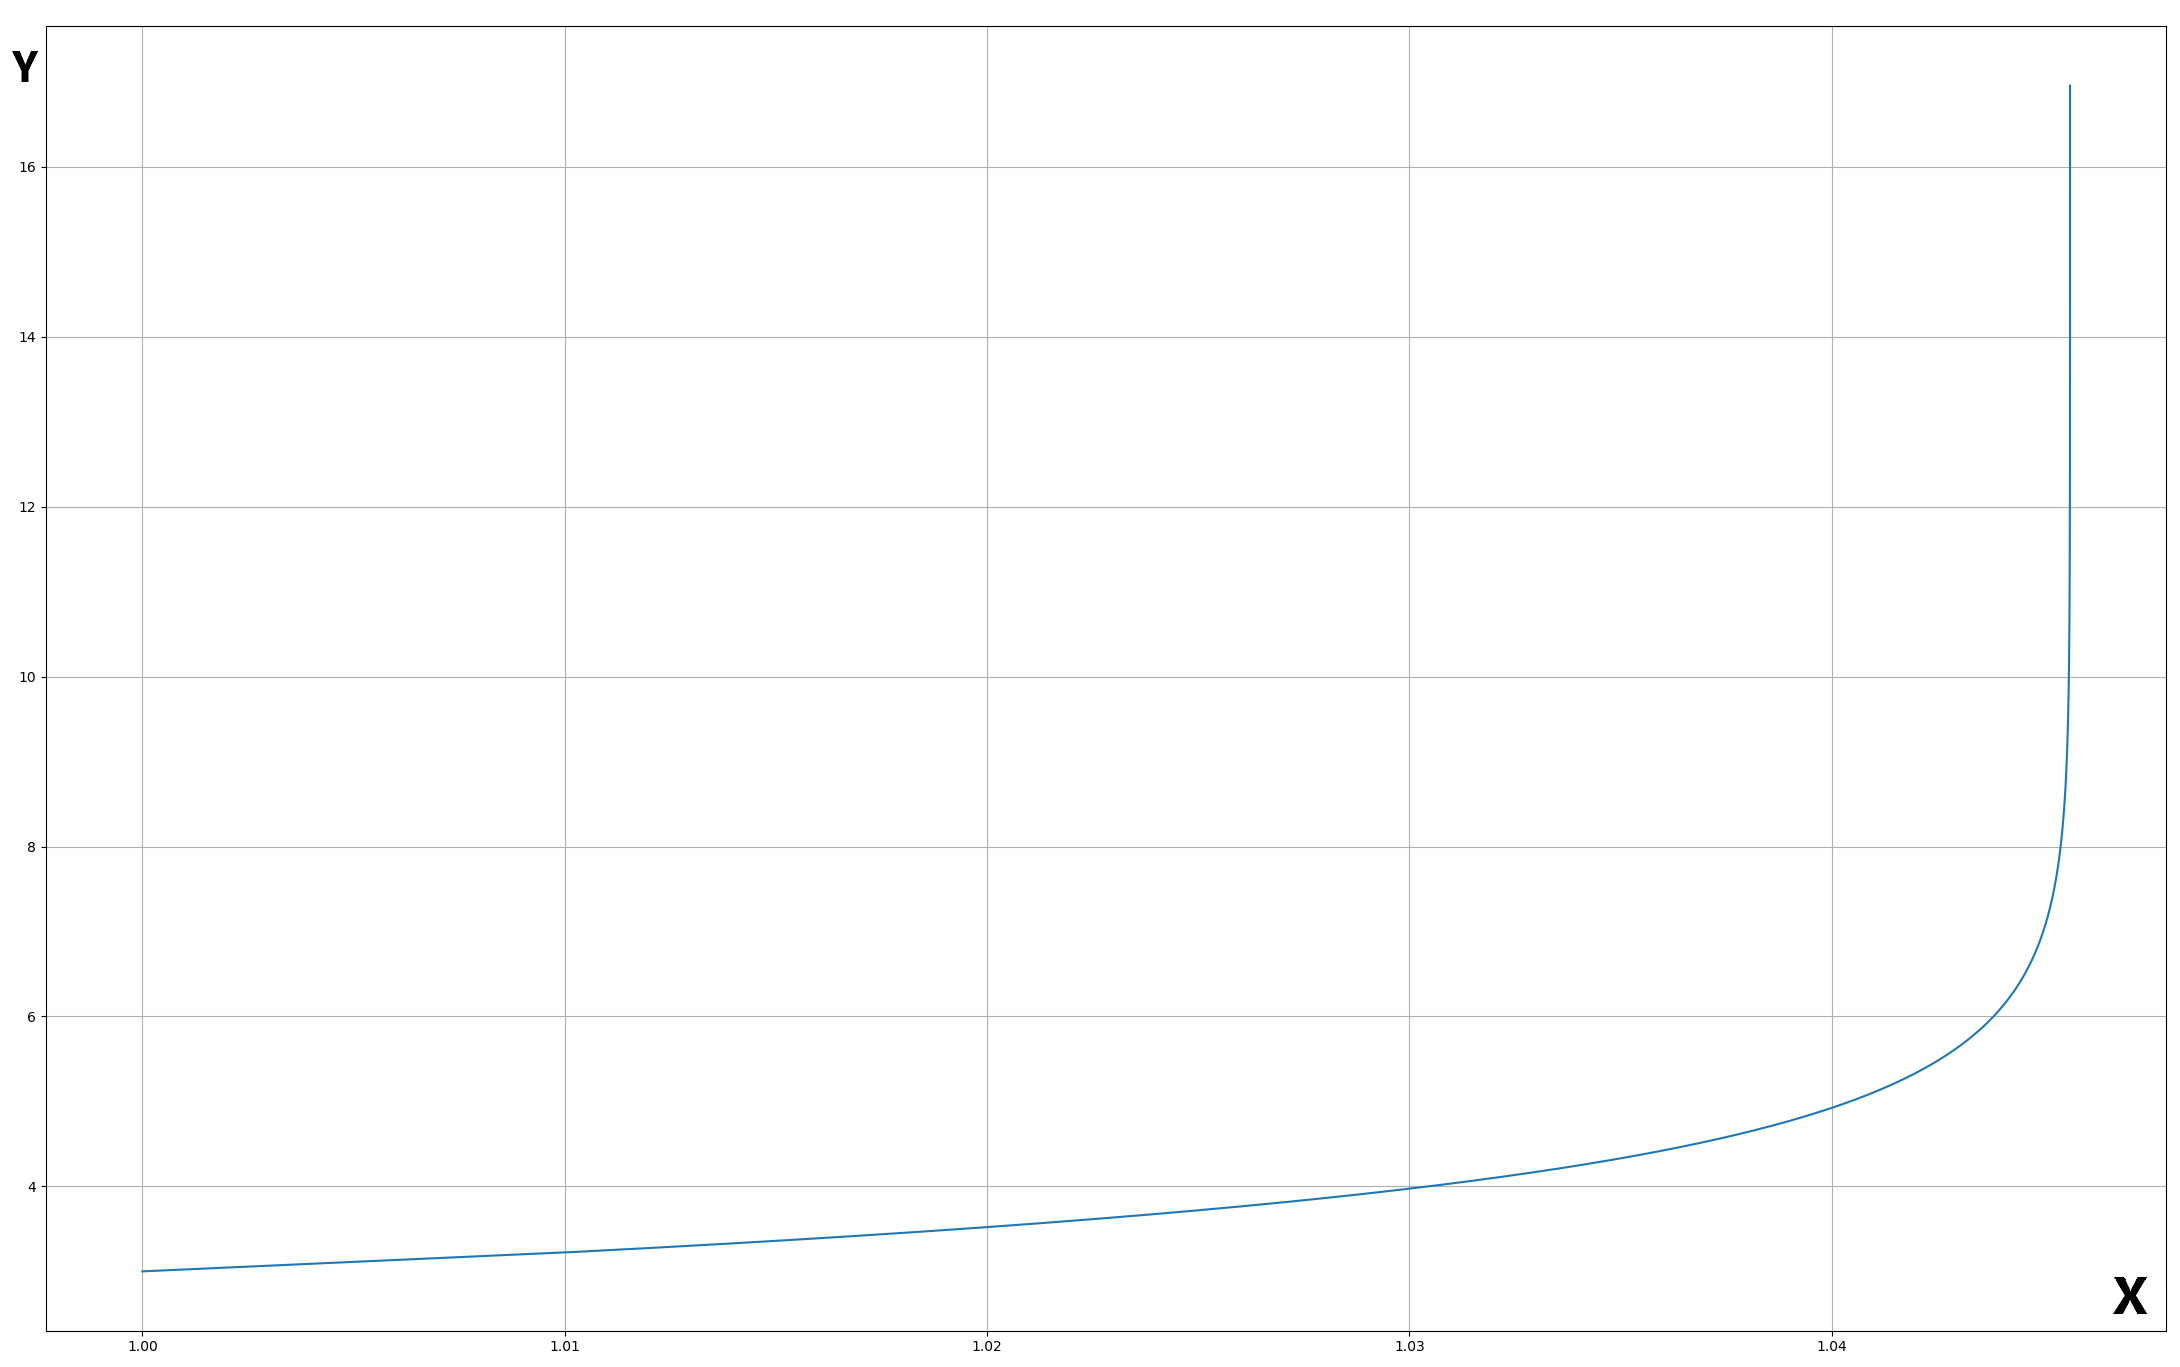
\includegraphics[width = 15cm, height = 7cm]{Figure.png}
	\caption{微分方程数值解局部性质图示} \label{figure.label}
\end{figure}
	
\section*{分析}
	\noindent 一、程序终止原因
	
	方程步进求解过程最后的终止点大约为 $(x,\,y) = (1.0456,\,678.7980)$。抛出异常时,在该点计算的 $e^{xy} = 1.7953 \times 10^{308}$,numpy.float64 所能表示的最大数值约为 $1.7977 \times 10^{308}$,故有很大把握断定程序的终止正是因为 $e^{xy}$ 数值溢出。
	
	\noindent 二、步长公式
	
	采用的步长递推式
	\begin{equation}
		h \leftarrow 0.9 h\left(\dfrac{\delta}{|e|}\right)^{\frac{1}{1+p}}
	\end{equation}
	
	其中 $p = 5$。这导致 $|e| < 1.8817\delta$ 时步长增大;$|e| > 1.8817\delta$ 时步长减小。相比于将步长直接加倍或减半,该策略看起来要温和许多。若认为 $e = Ch^{1+p}$,递推式中的指数 $\dfrac{1}{1 + p}$ 便很容易理解。另外,为防止步进第一步误差过大,实际代码中第一步长并未采用给定的 $h_0 = 0.01$,而是用它进行尝试计算,得到的 $h_1$ 将作为第一步长。
	


\section*{工作环境}
	程序所用语言: {\bf python}
	
	软件: {\bf JupyterLab}
	
	使用的包: {\bf numpy,matplotlib,bisect,warnings,traceback}

	
\section*{参考资料}
	\noindent [1] David R. Kincaid \& E. Ward Cheney. {\it Numerical Analysis: Mathematics of Scientific of Computing Third Edition}, Brooks/Cole, 2002.

\end{document}